\documentclass[10pt,a4paper]{ctexart}
\usepackage[margin=2cm]{geometry}
\usepackage{graphicx}
\usepackage{float}      % 支持 [H] 浮动体选项
\usepackage{hyperref}
\usepackage{amsmath}    % 提供方程环境
\usepackage{physics}    % 简化向量、微分算子语法
\newcommand{\myspace}[1]{\par\vspace{#1\baselineskip}} %自定义空一行
\usepackage{fancyhdr}
\pagestyle{fancy}
\fancyhf{}  % 清除所有页眉页脚
\fancyfoot[C]{\thepage}  % 在页脚中央设置页码
\renewcommand{\headrulewidth}{0pt}  % 去掉页眉横线
\renewcommand{\footrulewidth}{0pt}  % 去掉页脚横线

\usepackage{hyperref}
\hypersetup{
    colorlinks=true,
    linkcolor=blue,
    filecolor=magenta,      
    urlcolor=cyan,
    pdftitle={Overleaf Example},
    pdfpagemode=FullScreen,
    }

\usepackage{titlesec}

% 重新定义section格式
\titleformat{\section}
  {\normalfont\Large\bfseries}
  {\chinese{section}、}
  {0pt}
  {}

% 给出常用字号的自定义指令
\newcommand{\chuhao}{\fontsize{42pt}{48pt}\selectfont}
\newcommand{\xiaochu}{\fontsize{36pt}{42pt}\selectfont}
\newcommand{\xiaoer}{\fontsize{18pt}{21.6pt}\selectfont}
\newcommand{\sanhao}{\fontsize{16pt}{20pt}\selectfont}
\newcommand{\xiaosan}{\fontsize{15pt}{18pt}\selectfont}
\newcommand{\sihao}{\fontsize{14pt}{18pt}\selectfont}
\newcommand{\xiaosi}{\fontsize{12pt}{16pt}\selectfont}
\newcommand{\wuhao}{\fontsize{10.5pt}{12.6pt}\selectfont}

% 定义中文数字转换
\titleformat{\section}
  {\normalfont\Large\bfseries}
  {\zhnum{section}、}  % 使用\zhnum而不是\chinese
  {0pt}
  {}

% 标题设置
\title{\xiaochu\textbf{物理实验预习报告}}
\author{}
\date{}

\begin{document}

\vspace*{36pt} % 顶部空白

% 居中填写区域
\begin{center}   
    \xiaochu\textbf{物理实验预习报告}
    % 预留空白区域
    \vspace{13pt}
    \vspace{13pt}
    \vspace{13pt}
    \vspace{13pt}
    
    \sanhao\textbf{实验名称：\underline{\makebox[10cm]{ 光的偏振研究}}} \\[10pt]
    \sanhao\textbf{指导教师：\underline{\makebox[10cm]{ 姜柏旭 }}} \\[30pt]
    
    % 预留空白区域
    \myspace{6}
    
   \sihao\textbf{班级：\underline{\makebox[6cm]{}}} \\[10pt]
    \sihao\textbf{姓名：\underline{\makebox[6cm]{}}} \\[10pt]
    \sihao\textbf{学号：\underline{\makebox[6cm]{}}} \\[30pt]
    
   \sihao\textbf{实验日期: 
   \underline{\makebox[0.8cm]{2025}}  年 
   \underline{\makebox[0.4cm]{12}}月
   \underline{\makebox[0.4cm]{3}}日  
   星期\underline{\makebox[0.6cm]{三}}上午}
    
    \vspace{18pt}
    \sihao 浙江大学物理实验教学中心
    
\end{center}

\newpage

    \section{实验综述}
    
    \xiaosi （自述实验现象、实验原理和实验方法，不超过300字，5分）

    光虽然本质是电磁波，有电场和磁场两个分矢量，但是引起视觉效应的主要是电场矢量的振动方向。
    自然光的电场矢量在垂直于传播方向的各个方向上均匀振动，称为非偏振光；
    如果电场矢量只在某一特定方向上振动，则称为偏振光。
    偏振光可以通过反射、折射、散射等方法产生，也可以通过一些光学器件如偏振片、双折射晶体等获得。

    反射产生的偏振光现象称为布儒尔偏振现象，当光线以某一特定角度（布儒斯特角）入射到介质界面时，反射光完全偏振并与折射光垂直。
    本实验通过如下图的实验装置观察布儒尔偏振现象，测量布儒斯特角并得到介质的折射率；

\begin{figure}[H]
    \centering
    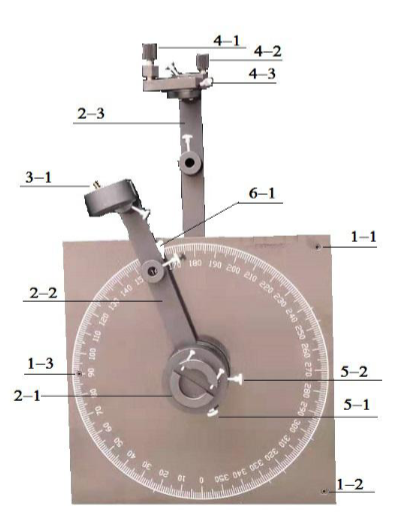
\includegraphics[width=0.6\textwidth]{figure/ex.png}
    \caption{布儒尔偏振现象实验装置示意图}
\end{figure}
    之后通过使光线以布儒斯特角入射，调整偏振片的转动角度，使光强出现极大和极小来测量偏振片的偏振化方向角度。
\myspace{2}
    
实验通过改变偏振片角度和测量光强的关系，验证马吕斯定律，即通过偏振片后的光强与入射光强和偏振片夹角的平方成正比关系并研究硅光电池的光电流和光强的关系。
    \section{实验重点}
    
    \xiaosi（简述本实验的学习重点，不超过100字，3分）

    (1)利用布儒斯特角测量黑色平板折射率

    (2)测量偏振片的偏振化方向角度

    (3)验证马吕斯定律,研究硅光电池的光电流和光强的关系
    \myspace{2}
    
    \section{实验难点}

    \xiaosi（简述本实验的实现难点，不超过100字，2分）

    (1)调节光路，使入射光线以布儒斯特角入射到介质界面；

    (2)准确测量偏振片的偏振化方向角度；

    (3)验证马吕斯定律时，准确测量不同偏振片角度下的光强值。

    (4)调整器件等高共轴
    
    (5)测量折射率时准确确定光强最小的角度
\myspace{2}


\newpage

\sihao\textbf{注意事项：}
\xiaosi
\begin{enumerate}
    \item 用PDF格式上传“预习报告”，文件名：学生姓名+学号+实验名称+周次。
    \item “预习报告”必须递交在“学在浙大”的本课程的对应实验项目的“作业”模块内。
    \item “预习报告”还须拷贝到“实验报告”中（便以教师批改）。
    \item 大学物理实验”课程选做实验使用本“预习报告”；必做实验无须写预习报告，前往“学在浙大”完成预习测试即可。
\end{enumerate}

\vspace{1cm}
\xiaosi\centering \textbf{浙江大学物理实验教学中心制}

\end{document}
